\documentclass{standalone}
\usepackage{tikz}
\usetikzlibrary{patterns, positioning}
\usetikzlibrary{shapes.misc}
\usepackage[outline]{contour}
\contourlength{1.5pt} 


\begin{document}
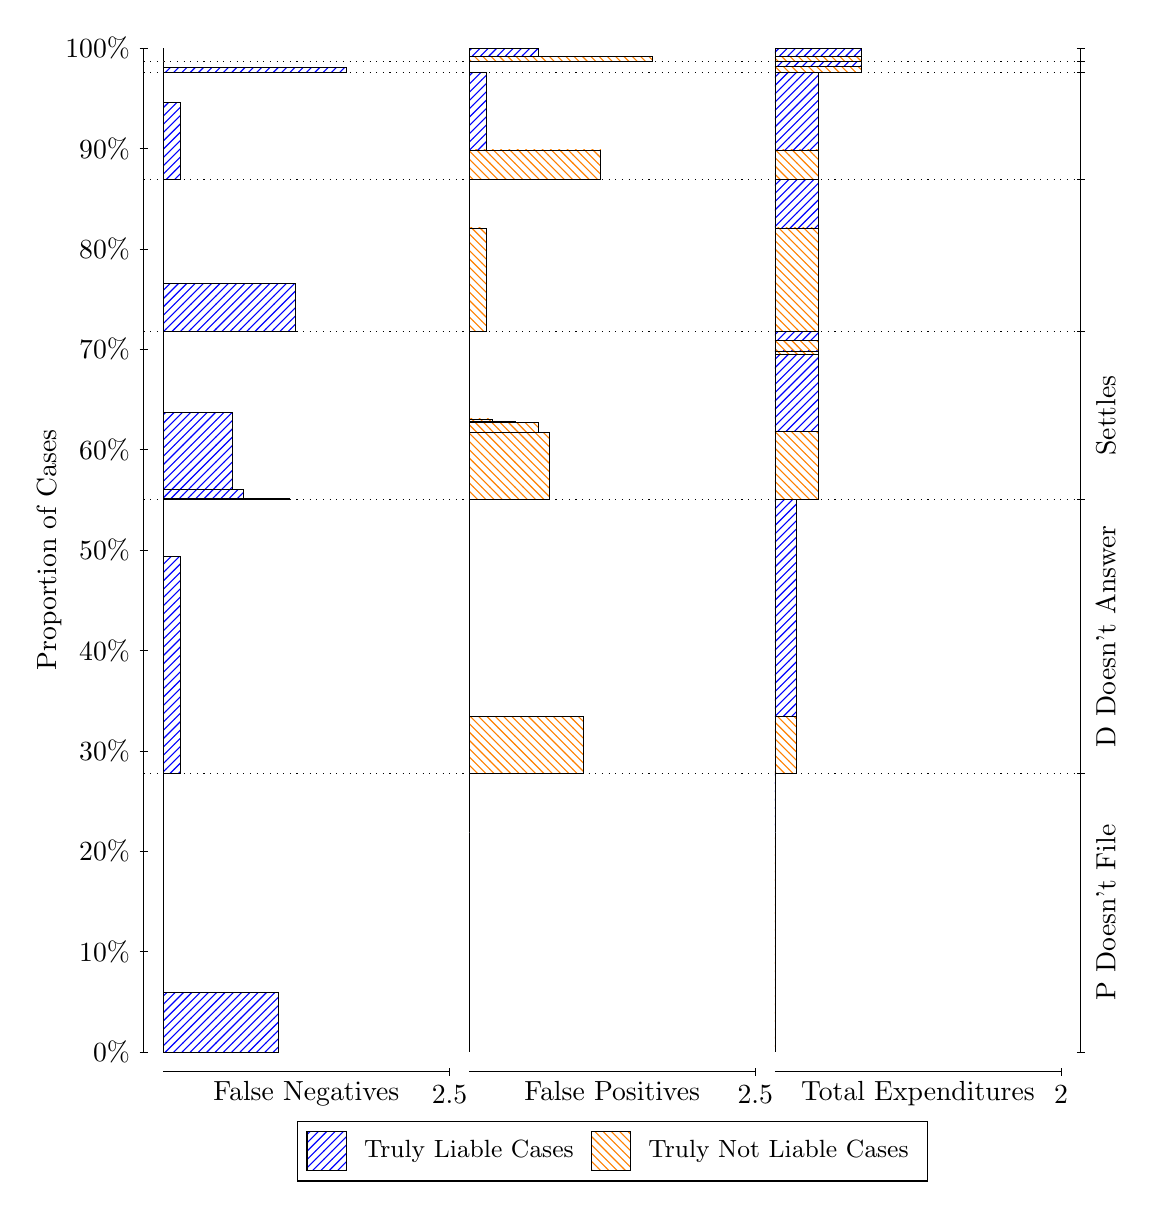
\begin{tikzpicture}
\draw[black, very thin] (1.5,1.75) -- (1.5,14.5);
\node[rotate=90, text=black, anchor=center] at (0.3, 8.125) {Proportion of Cases};
\draw[black, very thin] (1.45,1.75) -- (1.55,1.75);
\node[text=black, anchor=east] at (1.45, 1.75) {0\%};
\draw[black, very thin] (1.45,3.025) -- (1.55,3.025);
\node[text=black, anchor=east] at (1.45, 3.025) {10\%};
\draw[black, very thin] (1.45,4.3) -- (1.55,4.3);
\node[text=black, anchor=east] at (1.45, 4.3) {20\%};
\draw[black, very thin] (1.45,5.575) -- (1.55,5.575);
\node[text=black, anchor=east] at (1.45, 5.575) {30\%};
\draw[black, very thin] (1.45,6.85) -- (1.55,6.85);
\node[text=black, anchor=east] at (1.45, 6.85) {40\%};
\draw[black, very thin] (1.45,8.125) -- (1.55,8.125);
\node[text=black, anchor=east] at (1.45, 8.125) {50\%};
\draw[black, very thin] (1.45,9.4) -- (1.55,9.4);
\node[text=black, anchor=east] at (1.45, 9.4) {60\%};
\draw[black, very thin] (1.45,10.675) -- (1.55,10.675);
\node[text=black, anchor=east] at (1.45, 10.675) {70\%};
\draw[black, very thin] (1.45,11.95) -- (1.55,11.95);
\node[text=black, anchor=east] at (1.45, 11.95) {80\%};
\draw[black, very thin] (1.45,13.225) -- (1.55,13.225);
\node[text=black, anchor=east] at (1.45, 13.225) {90\%};
\draw[black, very thin] (1.45,14.5) -- (1.55,14.5);
\node[text=black, anchor=east] at (1.45, 14.5) {100\%};

\draw[black, very thin] (13.4,1.75) -- (13.4,14.5);
\draw[black, very thin] (13.35,1.75) -- (13.45,1.75);
\node[anchor=west] at (13.35, 1.75) {};
\draw[black, very thin] (13.35,5.2922) -- (13.45,5.2922);
\node[anchor=west] at (13.35, 5.2922) {};
\draw[black, very thin] (13.35,8.7693) -- (13.45,8.7693);
\node[anchor=west] at (13.35, 8.7693) {};
\draw[black, very thin] (13.35,10.897) -- (13.45,10.897);
\node[anchor=west] at (13.35, 10.897) {};
\draw[black, very thin] (13.35,12.828) -- (13.45,12.828);
\node[anchor=west] at (13.35, 12.828) {};
\draw[black, very thin] (13.35,14.19) -- (13.45,14.19);
\node[anchor=west] at (13.35, 14.19) {};
\draw[black, very thin] (13.35,14.331) -- (13.45,14.331);
\node[anchor=west] at (13.35, 14.331) {};
\draw[black, very thin] (13.35,14.5) -- (13.45,14.5);
\node[anchor=west] at (13.35, 14.5) {};

\draw[black, very thin, pattern color=blue, pattern=north east lines] (1.75,1.75) rectangle (3.2033,2.5051);
\draw[black, very thin, pattern color=orange, pattern=north west lines] (1.75,2.5051) rectangle (1.75,5.2922);
\draw[black, very thin, pattern color=blue, pattern=north east lines] (1.75,5.2922) rectangle (1.968,8.0462);
\draw[black, very thin, pattern color=orange, pattern=north west lines] (1.75,8.0462) rectangle (1.75,8.7693);
\draw[black, very thin, pattern color=blue, pattern=north east lines] (1.75,8.7693) rectangle (3.3487,8.777);
\draw[black, very thin, pattern color=blue, pattern=north east lines] (1.75,8.777) rectangle (3.058,8.7832);
\draw[black, very thin, pattern color=blue, pattern=north east lines] (1.75,8.7832) rectangle (2.7673,8.8948);
\draw[black, very thin, pattern color=blue, pattern=north east lines] (1.75,8.8948) rectangle (2.622,9.8755);
\draw[black, very thin, pattern color=orange, pattern=north west lines] (1.75,9.8755) rectangle (1.75,10.897);
\draw[black, very thin, pattern color=blue, pattern=north east lines] (1.75,10.897) rectangle (3.4213,11.508);
\draw[black, very thin, pattern color=orange, pattern=north west lines] (1.75,11.508) rectangle (1.75,12.828);
\draw[black, very thin, pattern color=blue, pattern=north east lines] (1.75,12.828) rectangle (1.968,13.811);
\draw[black, very thin, pattern color=orange, pattern=north west lines] (1.75,13.811) rectangle (1.75,14.19);
\draw[black, very thin, pattern color=blue, pattern=north east lines] (1.75,14.19) rectangle (4.0753,14.251);
\draw[black, very thin, pattern color=orange, pattern=north west lines] (1.75,14.251) rectangle (1.75,14.331);
\draw[black, very thin, pattern color=orange, pattern=north west lines] (1.75,14.331) rectangle (1.75,14.397);
\draw[black, very thin, pattern color=blue, pattern=north east lines] (1.75,14.397) rectangle (1.75,14.5);
\draw[black, very thin, pattern color=orange, pattern=north west lines] (5.6333,1.75) rectangle (5.6333,4.5371);
\draw[black, very thin, pattern color=blue, pattern=north east lines] (5.6333,4.5371) rectangle (5.6333,5.2922);
\draw[black, very thin, pattern color=orange, pattern=north west lines] (5.6333,5.2922) rectangle (7.0867,6.0153);
\draw[black, very thin, pattern color=blue, pattern=north east lines] (5.6333,6.0153) rectangle (5.6333,8.7693);
\draw[black, very thin, pattern color=orange, pattern=north west lines] (5.6333,8.7693) rectangle (6.6507,9.6148);
\draw[black, very thin, pattern color=orange, pattern=north west lines] (5.6333,9.6148) rectangle (6.5053,9.7471);
\draw[black, very thin, pattern color=orange, pattern=north west lines] (5.6333,9.7471) rectangle (6.2147,9.7594);
\draw[black, very thin, pattern color=orange, pattern=north west lines] (5.6333,9.7594) rectangle (5.924,9.7905);
\draw[black, very thin, pattern color=blue, pattern=north east lines] (5.6333,9.7905) rectangle (5.6333,10.897);
\draw[black, very thin, pattern color=orange, pattern=north west lines] (5.6333,10.897) rectangle (5.8513,12.216);
\draw[black, very thin, pattern color=blue, pattern=north east lines] (5.6333,12.216) rectangle (5.6333,12.828);
\draw[black, very thin, pattern color=orange, pattern=north west lines] (5.6333,12.828) rectangle (7.3047,13.206);
\draw[black, very thin, pattern color=blue, pattern=north east lines] (5.6333,13.206) rectangle (5.8513,14.19);
\draw[black, very thin, pattern color=orange, pattern=north west lines] (5.6333,14.19) rectangle (5.6333,14.27);
\draw[black, very thin, pattern color=blue, pattern=north east lines] (5.6333,14.27) rectangle (5.6333,14.331);
\draw[black, very thin, pattern color=orange, pattern=north west lines] (5.6333,14.331) rectangle (7.9587,14.397);
\draw[black, very thin, pattern color=blue, pattern=north east lines] (5.6333,14.397) rectangle (6.5053,14.5);
\draw[black, very thin, pattern color=orange, pattern=north west lines] (9.5167,1.75) rectangle (9.5167,4.5371);
\draw[black, very thin, pattern color=blue, pattern=north east lines] (9.5167,4.5371) rectangle (9.5167,5.2922);
\draw[black, very thin, pattern color=orange, pattern=north west lines] (9.5167,5.2922) rectangle (9.7892,6.0153);
\draw[black, very thin, pattern color=blue, pattern=north east lines] (9.5167,6.0153) rectangle (9.7892,8.7693);
\draw[black, very thin, pattern color=orange, pattern=north west lines] (9.5167,8.7693) rectangle (10.062,9.6271);
\draw[black, very thin, pattern color=blue, pattern=north east lines] (9.5167,9.6271) rectangle (10.062,10.614);
\draw[black, very thin, pattern color=orange, pattern=north west lines] (9.5167,10.614) rectangle (10.062,10.645);
\draw[black, very thin, pattern color=blue, pattern=north east lines] (9.5167,10.645) rectangle (10.062,10.653);
\draw[black, very thin, pattern color=orange, pattern=north west lines] (9.5167,10.653) rectangle (10.062,10.785);
\draw[black, very thin, pattern color=blue, pattern=north east lines] (9.5167,10.785) rectangle (10.062,10.897);
\draw[black, very thin, pattern color=orange, pattern=north west lines] (9.5167,10.897) rectangle (10.062,12.216);
\draw[black, very thin, pattern color=blue, pattern=north east lines] (9.5167,12.216) rectangle (10.062,12.828);
\draw[black, very thin, pattern color=orange, pattern=north west lines] (9.5167,12.828) rectangle (10.062,13.206);
\draw[black, very thin, pattern color=blue, pattern=north east lines] (9.5167,13.206) rectangle (10.062,14.19);
\draw[black, very thin, pattern color=orange, pattern=north west lines] (9.5167,14.19) rectangle (10.607,14.27);
\draw[black, very thin, pattern color=blue, pattern=north east lines] (9.5167,14.27) rectangle (10.607,14.331);
\draw[black, very thin, pattern color=orange, pattern=north west lines] (9.5167,14.331) rectangle (10.607,14.397);
\draw[black, very thin, pattern color=blue, pattern=north east lines] (9.5167,14.397) rectangle (10.607,14.5);
\draw[black, dotted] (1.5,5.2922) -- (13.4,5.2922);
\draw[black, dotted] (1.5,8.7693) -- (13.4,8.7693);
\draw[black, dotted] (1.5,10.897) -- (13.4,10.897);
\draw[black, dotted] (1.5,12.828) -- (13.4,12.828);
\draw[black, dotted] (1.5,14.19) -- (13.4,14.19);
\draw[black, dotted] (1.5,14.331) -- (13.4,14.331);
\draw[black, very thin] (1.75,1.5) -- (5.3833,1.5);
\node[text=black, anchor=north] at (3.5667, 1.5) {False Negatives};
\draw[black, very thin] (5.3833,1.45) -- (5.3833,1.55);
\node[text=black, anchor=north] at (5.3833, 1.45) {2.5};

\draw[black, very thin] (5.6333,1.5) -- (9.2667,1.5);
\node[text=black, anchor=north] at (7.45, 1.5) {False Positives};
\draw[black, very thin] (9.2667,1.45) -- (9.2667,1.55);
\node[text=black, anchor=north] at (9.2667, 1.45) {2.5};

\draw[black, very thin] (9.5167,1.5) -- (13.15,1.5);
\node[text=black, anchor=north] at (11.333, 1.5) {Total Expenditures};
\draw[black, very thin] (13.15,1.45) -- (13.15,1.55);
\node[text=black, anchor=north] at (13.15, 1.45) {2};

\node[text=black, centered, rotate=90] at (13.72, 3.5211) {\contour{white}{P Doesn't File}};
\node[text=black, centered, rotate=90] at (13.72, 7.0308) {\contour{white}{D Doesn't Answer}};
\node[text=black, centered, rotate=90] at (13.72, 9.833) {\contour{white}{Settles}};





\draw (7.449999999999999,1.5) node[draw=none] (baseCoordinate) {};
\begin{scope}[align=center]
        \matrix[scale=0.5, draw=black, below=0.5cm of baseCoordinate, nodes={draw}, column sep=0.1cm]{
            \node[rectangle, draw, minimum width=0.5cm, minimum height=0.5cm, pattern color=blue, pattern=north east lines] {}; &
            \node[draw=none, font=\small, text=black] (B) {Truly Liable Cases}; &
            \node[rectangle, draw, minimum width=0.5cm, minimum height=0.5cm, pattern color=orange, pattern=north west lines] {}; &
            \node[draw=none, font=\small, text=black] (B) {Truly Not Liable Cases}; \\
            };
\end{scope}

\end{tikzpicture}
\end{document}